\section{System Overview}\label{chapter.system_overview}
\thispagestyle{plain}

This chapter aims to provide an overview of how \toolname \space is assembled by describing the design and architecture of the system. System setup will be described thereafter, followed by a presentation of the web-based user interface of the tool.


\comment{
\info[inline]{[Frontend/On-Stage]

Detailed description of what the system does and how it works from the perspective of the user. Use edited screenshots with extra info and markings.

Don't add screenshots until the product is finished. This chapter should be around 10 pages or a little more (with screenshots)?}}





%%%%%%%%%%%%%%%%%%%%%%%%%%%%%%%%
% SUBSECTION: Architecture
%%%%%%%%%%%%%%%%%%%%%%%%%%%%%%%%
\subsection{Architecture}

\comment{\improvement[inline]{Chart of system architecture? Yes.\\ Chart of data flow? Maybe? (Or next ch.)\\ Explain how components communicate? Or should that be in next chapter? *confused*}}

\begin{figure}[p]
    \centering
    \thisfloatpagestyle{empty}
    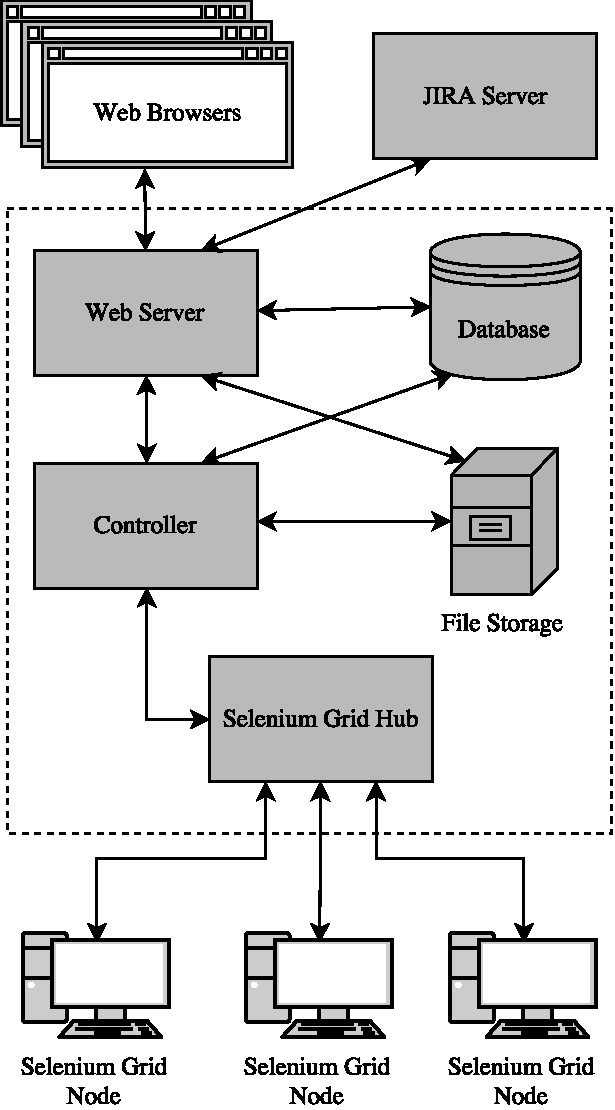
\includegraphics[height=\textheight]{figures/architecture.pdf}
    \caption{System Architecture}
    \label{fig.architecture}
\end{figure}

\toolname \space is operated through a web-based dashboard. This web service works as a content management system for test scripts. It allows for sending execution requests for the available test scripts, or for scheduling test runs ahead of time. 

Figure \ref{fig.architecture} shows the structural architecture of the system. In this case, the web server, the controller, the database, the file storage and the Selenium Grid Hub are all located on the same machine, hence the dashed border around these elements in the figure.

The web server uploads test scripts to a file location on the server. Meta data about the test cases as well as other information such as test groups, planned test executions, test results and user authentication are also stored in the database. The web server can report defects in the issue tracker system, which in the case of TV Overalt is JIRA.

The controller listens to test execution requests triggered through the dashboard. Upon an execution, it fetches the given test script from the file storage. Test scripts are sent to the current instance of the Selenium Grid Hub with specifications of which node in the distributed Selenium Grid that the test script should be executed on. The hub then triggers the given node to execute the test. After the test has finished, the controller stores the result in the database.







%%%%%%%%%%%%%%%%%%%%%%%%%%%%%%%%
% SUBSECTION: Setup
%%%%%%%%%%%%%%%%%%%%%%%%%%%%%%%%
\subsection{Setup}
\improvement[inline]{TODO}
\comment{\improvement[inline]{Explain how to set up the system?}
\info[inline]{Add a some customized VM ISO images to the thesis submission, each with different browsers installed. Preferably include a OSx VM. This subsection walks through how to set up the environment and start everything that needs to be started.}}









%%%%%%%%%%%%%%%%%%%%%%%%%%%%%%%%
% SUBSECTION: Dashboard
%%%%%%%%%%%%%%%%%%%%%%%%%%%%%%%%
\subsection{Dashboard}
The graphical user interface of \toolname \space is web-based, and is built on the high-level Web framework Django (\ref{subsection.django}). The framework provides a powerful automatic administrator interface, which has been used as a foundation for the development of the dashboard. Working with Django thus allowed for rapid development while retaining control of the content and functionality of the website. This was one of the main reasons why this particular framework was chosen for \toolname.

This subsection will present the dashboard from the user's perspective. An in-depth presentation of how some of the functionality has been implemented can be found in Chapter \ref{chapter.implementation}.

\comment{
\info[inline]{General explanation of how django change lists work? How attributes are chosen for listing, searching, filtering, that they are sortable. How object history works. Nah, maybe move that to implementation?}
}




%%%%%%%%%%%%
% SUBSUBSECTION: Home Screen
%%%%%%%%%%%%
\subsubsection{Home Screen}

\comment{\info[inline]{}}

\begin{figure}[h]
    \centering
    
\includegraphics[width=\textwidth]{figures/placeholder.png}
    \caption{Home Screen}
    \label{fig.home}
\end{figure}
\noindent
After logging in, the home screen is the first thing that meets the eye of the user. This screen provides navigation to all of the modules and pages described in the remaining subsections of this section. In order to give the user an indication of status, some graphs that show the results of recent test runs, as well as key numbers and other important information is displayed on this page.


%%%%%%%%%%%%
% SUBSUBSECTION: Authentication and Authorization
%%%%%%%%%%%%
\subsubsection{Authentication \& Authorization}

\comment{
\unsure[inline]{Some gamification element might be added, in which case this module must be customized, and screenshots must be provided.}
}

\begin{figure}[h]
    \centering
    
\includegraphics[width=\textwidth]{figures/placeholder.png}
    \caption{Authentication and Authorization Module}
    \label{fig.tc_mod}
\end{figure}

\noindent The Django administrator interface provides some built-in functionality, including a module for authentication and authorization of users. \emph{Superusers} can list, edit and create new user accounts. They can also change user info and the permissions of other user accounts, add them to user groups, and specify the permissions of user accounts.

\toolname \space is a tool that is meant to be part of a business process in which only trusted peers should be allowed to take part, and by extension, \toolname \space should only be operated by trusted associates. For this reason, no user accounts can be created by anyone other than a superuser. Thus, any person who wants and account must request this by someone with superuser privileges. 

By default, all passwords are encrypted before being stored in the database.






%%%%%%%%%%%%
% SUBSUBSECTION: Settings/Configuration
%%%%%%%%%%%%
\subsubsection{Settings/Configuration}

\improvement[inline]{TODO}






%%%%%%%%%%%%
% SUBSUBSECTION: Test Case Module
%%%%%%%%%%%%
\subsubsection{Test Case Module}

\begin{figure}[h]
    \centering
    
\includegraphics[width=\textwidth]{figures/placeholder.png}
    \caption{Test Case Module}
    \label{fig.tc_mod}
\end{figure}

All registered test cases are listed in this module. The list contains meta data about the test cases as well as some values that are retrieved or calculated using information from other tables in the database. This includes the number of times the test case has been executed, the average execution time, the result of the previous execution and when the test case was last executed. \comment{\info{Next planned execution might also be displayed here? Can't be \emph{that} difficult.}} It is possible to search and filter the list to narrow down the elements listed, and to sort the list by clicking on the attribute names in the table header.

New test cases can be created by clicking the button labeled \emph{Add Test Case} in the upper right of the view. This opens a new page with a form in which the test script can be uploaded and corresponding details about the test case can be filled in. Which groups the test case should be a member of can also be specified here. Test cases can be members of multiple groups, or none. After a test case has been created, it can be edited by clicking on the title of the test case in the test case list.

It is possible to select test cases and perform actions on them. The action options - \emph{Delete selected test cases} and \emph{Execute selected test cases} - are located in a dropdown menu above the test case list. The former is a built-in Django function which, after the user confirms deletion in and intermediate page, removes all meta data regarding the selected items from the database. The latter action is implemented for \toolname. The action takes the user to an intermediate page in which they can specify the platform and browsers the test cases should be executed on.

When an action has been performed, or attempted performed, a feedback message telling if the action was successful or not is displayed on the screen.

\comment{
\info[inline]{js must be extended to check which browsers/platforms are currently available and update each time a browser/platform is selected. Form validation must also be included (check if all platform/browser combinations are still available when Execute is pushed).}
}

\begin{figure}[h]
    \centering
    
\includegraphics[width=\textwidth]{figures/placeholder.png}
    \caption{Intermediate Page for Immediate Test Execution Requests}
    \label{fig.tc_intermediate}
\end{figure}

\subsubsection{Test Group Module}

Test groups are listed similar to individual test cases as described in the previous subsection. As with the test cases, group items can also be searched, filtered and sorted. Additionally, new groups can be created, and existing groups can be edited.

However, the group model is simpler than the test case model. The purpose of this model is to group together test cases that should preferably be executed in the same test run.

\subsubsection{Scheduling Module}

The scheduling module provides an interface for planning test runs in the future. As with the test cases and groups, schedules are also displayed in a list can be searched, filtered and sorted. Schedule objects can be created and changed. Additionally, the schedule list enables schedule objects to be activated and deactivated from the action menu. Only activated schedule objects will start test runs according to their specified time of execution. This is the default status, and deactivation of schedule objects must be appointed explicitly through the action menu.

\begin{figure}[h]
    \centering
    
\includegraphics[width=\textwidth]{figures/placeholder.png}
    \caption{Schedule Creation Form}
    \label{fig.sched_mod}
\end{figure}

Upon creating or editing a schedule object, an execution time can be specified along with any desired recurrence pattern along with the option of providing an end time. Test groups or individual test cases that should be included in the schedule object are also specified here.

\subsubsection{Execution Log}

\comment{\info[inline]{Include issue reporting to Jira}}

The layout of the log is the same as the remaining list views, but the functionality differs in that log items are read-only. They can not be created or deleted. Log items are created and inserted into the database based on the result from test executions. Each log object corresponds to an execution of an individual test script. The information listed in the logs include a number of attributes such as the duration of the test execution, the IP address or hostname of the machine on which it was executed, as well as information such as browser, platform, output and of course the result.







\subsubsection{Other}

\comment{\todo[inline]{TODO}}

\comment{\info[inline]{These pages contain how tos, different explanations of stuffs, where to find whatever, how to set up everything. About contains any necessary licenses (orbitron font, icons, etc.) and any other info about \toolname \space and maybe that it was lovingly created by me as my master's thesis?}}

\noindent The \betterfakesc{Help} page contains miscellaneous information regarding how \toolname \space works and how to use it. This page can be of help to technical testers who wants to use the tool, and otherwise to those who wants insight of how it works.

The \betterfakesc{About} page provides a short presentation what \toolname \space is and how it came to be. Any necessary licenses are also included in this page.